\lecture[
  date={September 27, 2021},
  author={M.J.W. Snippe},
  course={Example course with long name},
  course code={L.[bison-id]},
  short course={Short course},
]{Lecture name}

\section{First major topic}

  \subsection{Minor part of major topic}

    \begin{frame}{Frame title}
      \begin{itemize}
        \item You can use \texttt{\textbackslash insertsection} or \texttt{\textbackslash insertsubsection} to use respectively section or subsection titles as frame title.
      \end{itemize}
    \end{frame}

    \begin{frame}{Appearing bullet points}
      \begin{itemize}[<+- | alert@+>]
        \item Look at that
        \item I'm highlighted when appearing
        \item But only when using \texttt{make lecture-1-slides}
        \item Not when using \texttt{make lecture-1-handout}
      \end{itemize}
    \end{frame}

    \begin{frame}{Figure path}

      \begin{columns}
        \begin{column}{0.5\linewidth}
          \begin{figure}
            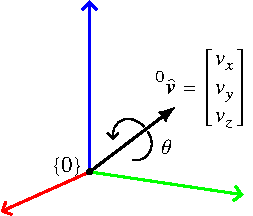
\includegraphics[width=0.7\linewidth]{axis-angle}
            \caption{Axis angle representation of 3D rotation.}
          \end{figure}
        \end{column}
        \begin{column}{0.5\linewidth}
          \begin{itemize}
            \item Default figure path includes \texttt{<repo-root>/course\_materials/figures}
          \end{itemize}
        \end{column}
      \end{columns}
      
    \end{frame}

    \begin{frame}[fragile]{Code: \matlab}
      
      \begin{block}{}
        \begin{matlabcode}
          T_1 = trot2(pi/6);
          T_2 = transl2(1,2);
          T_12 = T_1*T_2;
          T_21 = T_2*T_1;
          
          plotvol([-1 4 -1 4]);
          trplot2(T_1, 'frame', '1', 'color', 'b');
          trplot2(T_2, 'frame', '2', 'color', 'r');
          trplot2(T_12, 'frame', '12', 'color', 'g');
          trplot2(T_21, 'frame', '21', 'color', 'm');
        \end{matlabcode}
      \end{block}
      
    \end{frame}

    \mode<article>{
    Text here should only be added to the lecture notes document. Try \texttt{make lectures-notes} to compile lecture notes.
    }

    \begin{frame}[fragile]{Code: \python}
      
      \begin{block}{}
        \begin{pythoncode}
          import numpy as numpy

          def inv_SE3(T: np.array) -> np.array:
              """
              Inverts the transformation matrix T.
              """
              R = T[0:3, 0:3]
              p = T[0:3, 3:4]
          
              return R_p_to_SE3(R.T, np.dot(-R.T, p))
        \end{pythoncode}
      \end{block}
      
    \end{frame}